Para explicar los diferentes conceptos que se manejan en un árbol vamos a utilizar la siguiente representación que se muestra a continuación.

% TODO: \usepackage{graphicx} required
\begin{figure}[h!]
	\centering
	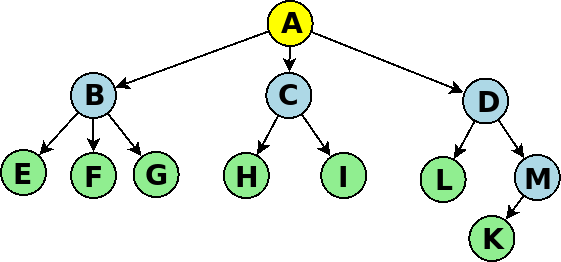
\includegraphics[width=0.7\linewidth]{img/tree_example}
	\label{fig:treeexample}
\end{figure}

\begin{itemize}
	\item \textbf{Nodos:} Se le llama nodo a cada elemento que contiene un árbol.
	
	\item \textbf{Nodo Raíz:} Se refiere al primer nodo de un árbol, solo un nodo del árbol puede ser la raíz (nodo de fondo amarillo). 
	
	\item \textbf{Nodo Padre:} Se utiliza este termino para llamar a todos aquellos nodos que tiene al menos un hijo (nodos de fondos amarillo y azules).
	
	\item \textbf{Nodo Hijo:} Los hijos son todos aquellos nodos que tiene un padre (nodos de fondo azul y verde).
	
	\item \textbf{Nodo Hermano:} Los nodos hermanos son aquellos nodos que comparte a un mismo padre en común dentro de la estructura. Los nodos $B$,$C$ y $D$ son hermanos, los nodos $E$,$F$ y $G$ también son hermanos.
	
	\item \textbf{Nodo Hoja:} Son todos aquellos nodos que no tienen hijos, los cuales siempre se encuentran en los extremos de la estructura (nodos de fondo verde).
	
	\item \textbf{Nodo Rama:} Estos son todos aquellos nodos que no son la raíz  y que además tiene al menos un hijo (nodos de fondos verdes).
\end{itemize}

Los árboles además de los nodos tiene otras propiedades importantes que son utilizadas en diferente ámbitos los cuales son:

\begin{itemize}
	\item \textbf{Nivel:} Nos referimos como nivel a cada generación dentro del árbol. Por ejemplo, cuando a un nodo hoja le agregamos un hijo, el nodo hoja pasa a ser un nodo rama pero además el árbol crece una generación por lo que el árbol tiene un nivel mas. Cada generación tiene un número de nivel distinto que las demas generaciones.
	
	\begin{itemize}
		\item Un árbol vacío tiene 0 niveles
		\item El nivel de la raíz es 1
		\item El nivel de cada nodo se calculado contando cuantos nodos existen sobre el, hasta llegar a la raíz + 1, y de forma inversa también se podría, contar cuantos nodos existes desde la raíz hasta el nodo buscado + 1.
	\end{itemize}

	El nodo $A$ tiene nivel 1. Con nivel 2 están los nodos $B$,$C$ y $D$ mientras el nodo $K$ tiene nivel 4 y el resto de los nodos sin mencionar nivel 3.

	\item \textbf{Altura:} Le llamamos altura al número máximo de niveles de un árbol. La altura es calculado mediante recursividad tomando el nivel mas grande de los dos sub-árboles de forma recursiva de la siguiente manera:
	$$ altura = max(altura(hijo1), altura(hijo2),altura(hijoN)) + 1 $$
	
	En el caso del árbol de ejemplo su altura es cuatro.
	
	\item \textbf{Peso:} Conocemos como peso a el número de nodos que tiene un Árbol. Este factor es importante por que nos da una idea del tamaño del árbol y el tamaño en memoria que nos puede ocupar en tiempo de ejecución(Complejidad Espacial en análisis de algoritmos.)
	
	El peso se puede calcular mediante cualquier tipo de recorrido el cual vaya contando los nodo a medida que avanza sobre la estructura. El peso es un árbol es igual a la suma del peso de los sub-árboles hijos + 1.
	
	$$ peso = peso(hijo1) + peso(hijo2) + peso(hijoN)+ 1 $$
	
	\item \textbf{Orden:} El orden de un árbol es el número máximo de hijos que puede tener un nodo. Notemos que un árbol con Orden = 1 no tendría sentido ya que seria una estructura lineal. Ya que cada nodo solo podría tener un hijo. Este valor no lo calculamos, si no que ya lo debemos conocer cuando diseñamos nuestra estructura, ya que si queremos calcular esto lo que obtendremos es el grado
	
	\item \textbf{Grado:} El grado se refiere al número mayor de hijos que tiene alguno de los nodos del árbol y esta limitado por el orden, ya que este indica el número máximo de hijos que puede tener un nodo.
	
	El grado se calcula contando de forma recursiva el número de hijos de cada sub-árbol hijo y el numero de hijos del nodo actual para tomar el mayor, esta operación se hace de forma recursiva para recorrer todo el árbol.
	
	$$ grado = max(contarHijos(hijo1),contarHijos(hijo2), contarHijos(hijoN), contarHijos(nodo)) $$
	
	\item \textbf{Sub-árbol:} Conocemos como sub-árbol a todo árbol generado a partir de una sección determinada del árbol, Por lo que podemos decir que un árbol es un nodo raíz con $N$ sub-árboles.
	
	Existen escenarios donde podemos sacar un Sub-Árboles del Árbol para procesarlo de forma separada, de esta forma el Sub-Árboles pasa a ser un Árbol independiente, También podemos eliminar Sub-Árboles completos, Agregarlos,entre otras operaciones. En árbol un posible subárbol sería el que conforman los nodos $B$, $E$, $F$ y $G$ donde el nodo B es la raiz.
	
	\item \textbf{Bosque:} Un bosque es un conjunto de árboles $n \ge 0 $ disjuntos.
	
	\item \textbf{Descendiente:} Un nodo accesible por descenso repetido de padre a hijo. Por ejemplo el nodo $K$ es descendiente del nodo $D$ mientras el nodo $F$ no es descendiente del nodo $D$.
	
	\item \textbf{Ancestro:} Un nodo accesible por ascenso repetido de hijo a padre. Por ejemplo el nodo $D$ es ancestro del nodo $K$ mientras el nodo $D$ no es ancestro del nodo $F$. 
	
	\item \textbf{Brazo:} La conexión entre un nodo y otro.
	
	\item \textbf{Camino:} Una secuencia de nodos y brazos conectados con un nodo descendiente. Un posible camimo es $D$,$M$ y $K$ no es un camino $B$,$A$ y $C$.
	
	\item \textbf{Longitud del camino:} Cantidad de nodos que se deben recorrer para llegar desde la raíz a un nodo determinado
	
	\item \textbf{Altura de un nodo:} La altura de un nodo es el número de brazos en el camino más largo entre ese nodo y una hoja.
	
	\item \textbf{Profundidad:} La profundidad de un nodo es el número de brazos desde la raíz del árbol hasta un nodo.
	
	
	
	\item \textbf{Rama:} Una ruta del nodo raíz a cualquier otro nodo.
\end{itemize}